% !TEX root = ../main.tex

% 中英标题:\chapter{中文标题}[英文标题]
\chapter{缺失值时间序列异常检测技术概述}[Typesetting pictures]

\section{引言}[Introduction]
本章是缺失值时间序列异常检测技术的相关理论基础。首先介绍了什么是时间序列中的异常,即时间序列异常的相关类型,包括点异常,上下文异常,集合异常和其他异常等。然后有关时间序列相关特性,即时间序列的相关属性,包括时序性,维度,非平稳性,噪声等属性。之后介绍了有关注意力机制相关技术,首先介绍了注意力机制的基本原理,然后介绍了注意力机制的计算方式及公式。最后介绍了标准化流的相关技术,包括当前主流实现标准化流的几种方式,即可加性耦合层,仿射耦合层等。

\section{时序数据的异常类型}[Doctoral picture example]
霍金斯\cite{hawkings}将异常值描述为一种与其他观察结果大相径庭的观察结果,以至于引起怀疑,认为它是由另一种机制产生的。在这种情况下,本文将时间序列数据中的异常描述为时间步骤中的数据点,这些数据点显示出与以前的时间步骤显著不同的意外行为。根据以往的文献,本文将与时间序列数据相关的异常分类如下。

点异常是突然偏离标准的数据点或序列。这样的异常似乎是时间噪声,通常是由传感器错误或异常系统操作引起的。为了进行检测,传统上设置了基于先前数据的上下控制限制,通常分别称为 UCL 和 LCL。这些极限之外存在的值被认为是点异常。
\begin{figure}[ht]
    \centering
    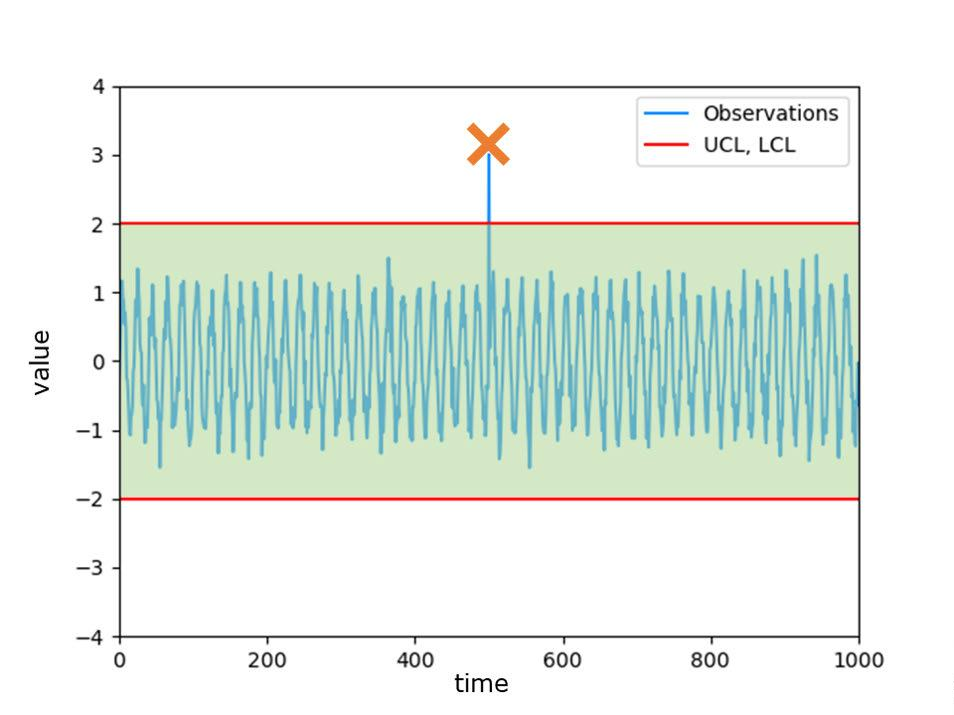
\includegraphics[width = 0.4\textwidth]{chapter2/point-anomaly.png}
    \caption{点异常}
    \end{figure}

与点异常类似,上下文异常表示在短时间内观察到的数据点或序列,但与预定义的 UCL 和 LCL 分界异常相同,不偏离正常范围。然而,考虑到给定的上下文 ,数据点脱离了预期的模式或形状。由于这个原因,这些异常可能很难检测到。
\begin{figure}[ht]
    \centering
    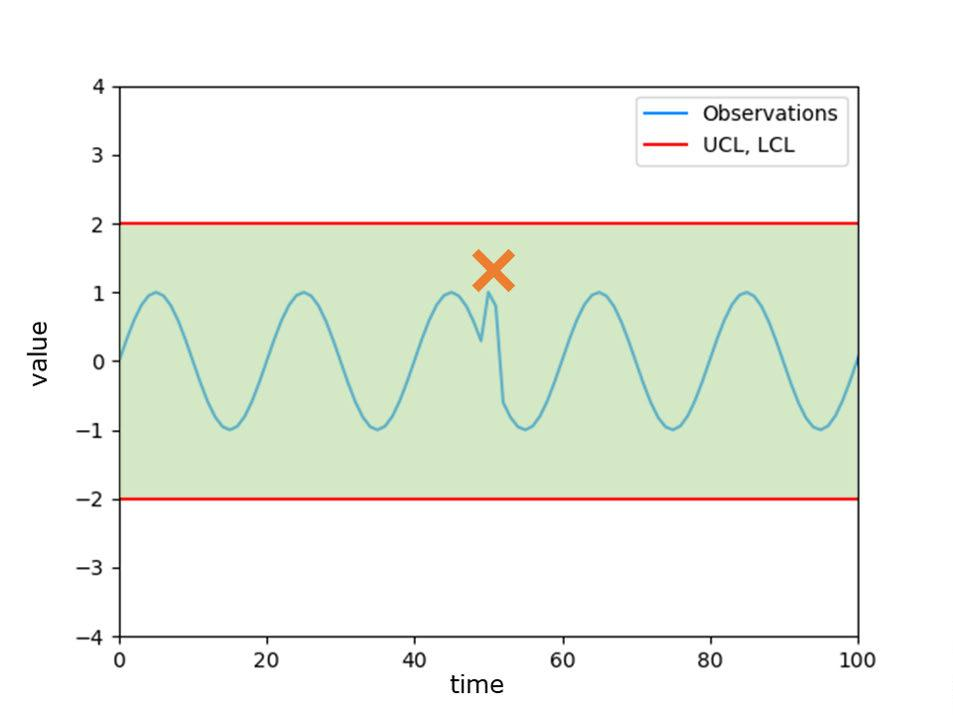
\includegraphics[width = 0.4\textwidth]{chapter2/context.png}
    \caption{上下文异常}
    \end{figure}

这种异常指的是一组数据点,这些数据点应该被视为异常,因为它们随着时间的推移逐渐显示出与正常数据不同的模式。这种异常类型中的个体价值观看起来似乎没有问题,但是作为一个整体,它们引起了怀疑。由于它们不容易一下子识别出来,所以从长远来看,上下文对于识别它们尤为重要。
\begin{figure}[ht]
    \centering
    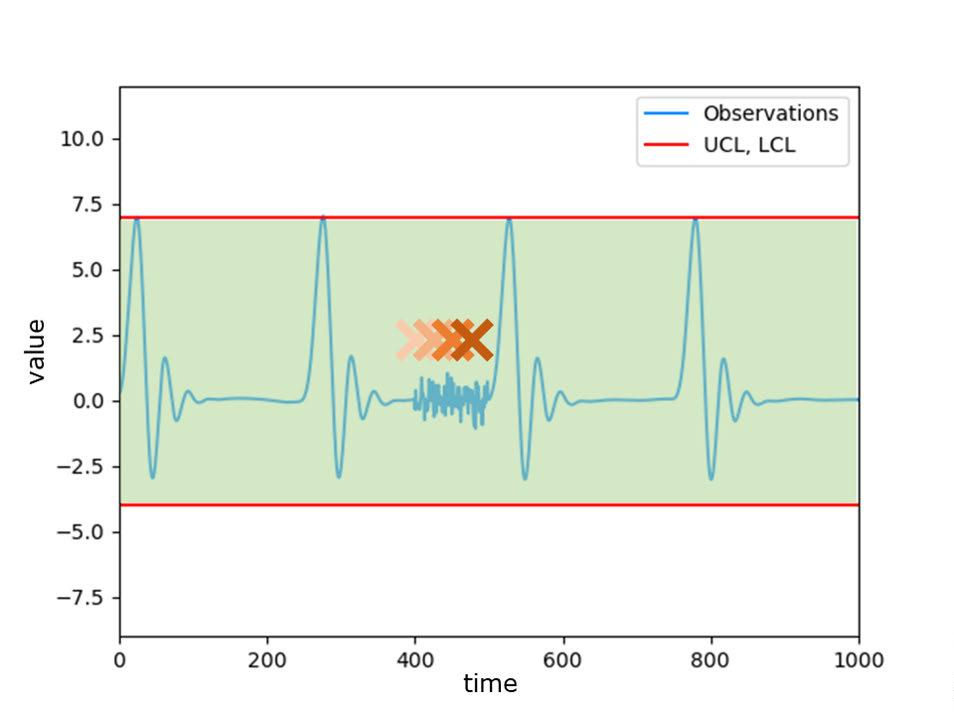
\includegraphics[width = 0.4\textwidth]{chapter2/colletective.png}
    \caption{上下文异常}
    \end{figure}

因为异常是正常状态之外的东西,所以什么是异常取决于对正常的定义。一般来说,异常可以分为上述三种类型之一,但其他观点可以细分为更具体的异常类别。

总之,异常是一种数据点,其发生在过去极为罕见,或者在逻辑上是不可能的。然而,在多变量时间序列数据中,可能不能像前面的例子那样对异常进行分类。多变量时间序列数据需要额外考虑变量与时间轴之间的关系。随着变量数量的增加,出现了更多多样化的模式。然后,异常模式可能是不规则的,并且正常状态和异常状态之间的差异可能是模糊的。扫描单个单变量时间序列数据并将其聚合以识别异常,并不能保证检测结果的准确性,因为很少有异常点会被其他正常变量掩盖,并对整个目标系统产生重大影响。通过提取清晰的变量或特征或使用足够复杂的模型来检测各种模式来减少维度可以解决这些问题。

\begin{figure}[htbp]
    \centering
    \subfigure{
    \begin{minipage}[t]{0.5\linewidth}
    \centering
    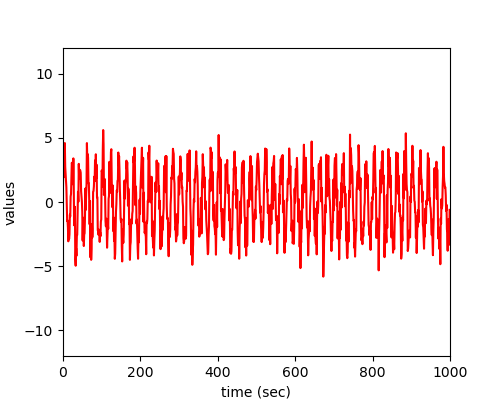
\includegraphics[width=2in]{chapter2/normal-1.png}
    \caption{正常时间序列}
    \end{minipage}%
    }%
    \subfigure{
    \begin{minipage}[t]{0.5\linewidth}
    \centering
    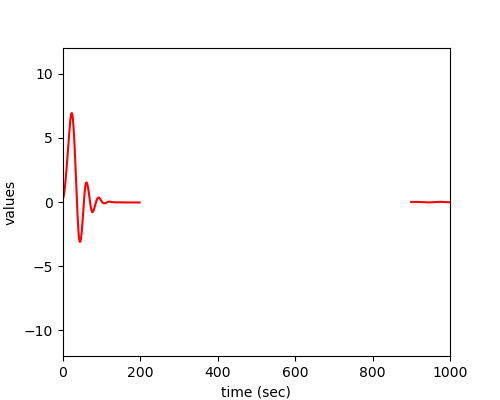
\includegraphics[width=2in]{chapter2/missing-2.png}
    \caption{数据丢失异常}
    \end{minipage}%
    }%
    % \subfigure{
    % \begin{minipage}[t]{0.25\linewidth}
    % \centering
    % 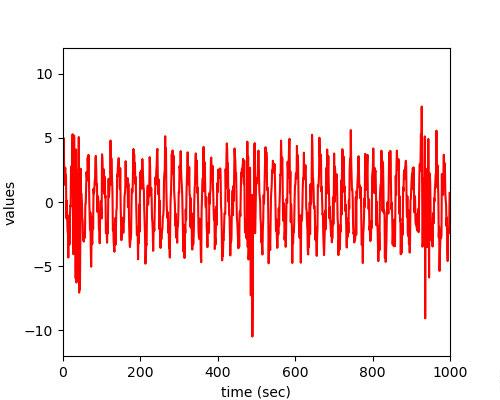
\includegraphics[width=1in]{chapter2/outlier-1.png}
    % \caption{数据点离群异常}
    % \end{minipage}
    % }%
    % \subfigure{
    % \begin{minipage}[t]{0.25\linewidth}
    % \centering
    % 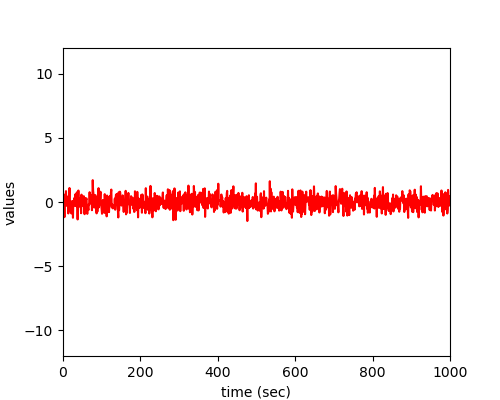
\includegraphics[width=1in]{chapter2/3-1.png}
    % \caption{时间序列频率异常}
    % \end{minipage}
    % }%
    \centering
    %\caption{其他异常举例}
    \end{figure}

\begin{figure}[htbp]
    \centering
    % \subfigure{
    % \begin{minipage}[t]{0.25\linewidth}
    % \centering
    % 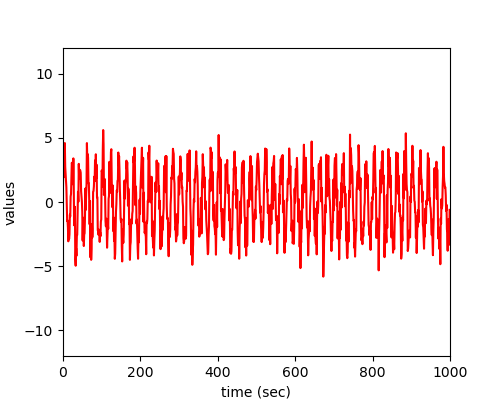
\includegraphics[width=1in]{chapter2/normal-1.png}
    % \caption{正常时间序列}
    % \end{minipage}%
    % }%
    % \subfigure{
    % \begin{minipage}[t]{0.25\linewidth}
    % \centering
    % 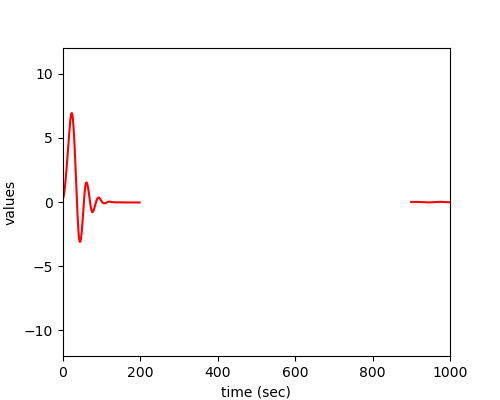
\includegraphics[width=1in]{chapter2/missing-2.png}
    % \caption{数据丢失异常}
    % \end{minipage}%
    % }%
    \subfigure{
    \begin{minipage}[t]{0.5\linewidth}
    \centering
    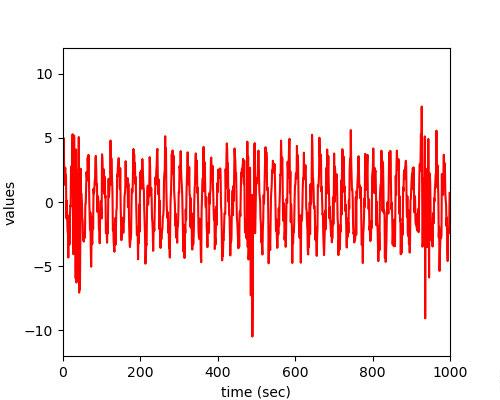
\includegraphics[width=2in]{chapter2/outlier-1.png}
    \caption{数据点离群异常}
    \end{minipage}
    }%
    \subfigure{
    \begin{minipage}[t]{0.5\linewidth}
    \centering
    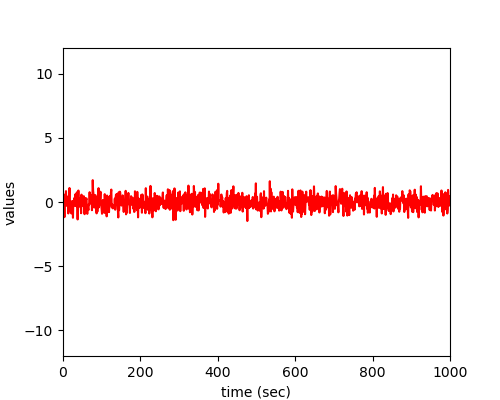
\includegraphics[width=2in]{chapter2/3-1.png}
    \caption{时间序列频率异常}
    \end{minipage}
    }%
    \centering
    %\caption{其他异常举例}
    \end{figure}

\section{时间序列相关属性}
虽然在几乎所有的任务中,时间都是一个基本概念,但处理时间敏感的数据需要仔细考虑。然而,如果很好地理解时间序列数据的特征,则可以通过利用来自信号的上下文信息来有效地检测异常。因此,我们简要描述了时间序列数据的基本原理。这里讨论的因素包括时间性、维数、非平稳性和噪声。

时间序列通常被认为是按时间顺序索引的观测值的集合。数据以相等的间隔捕获,序列中的每个连续数据点取决于其过去的值。因此,每个连续观测值之间存在一定的时间相关性或相关性[19]。观测序列的联合分布可以使用链积规则表示为。
\begin{equation}
	p\left(x^1, x^2, \ldots, x^T\right)=p\left(x^1\right) \prod_{t=2}^T p\left(x^t \mid x^1, x^2, \ldots, x^{t-1}\right)
	\end{equation}
其中 $x^t$ 是在时间 $t \in T \subseteq \mathbb{Z}^{+}$ 时观察到的数据点,每个条件概率 $p(\cdot \mid \cdot)$ 表示当前状态和以前状态之间的时间依赖关系。

维度是指每个观察中捕获的单个数据属性的数量\cite{yellow1}。根据维度,时间序列数据在很大程度上分为单变量和多变量类型。时间序列数据的维度影响计算成本和分析方法。单变量:这种类型描述了一组有序的实值观测值,其中每个数据点在一个特定的时间被测量,$t \in T \subseteq \mathbb{Z}^{+}$ 。然后,$x^t \in \mathbb{R}$ 是在时间 $t$ 处测量的数据点,是某个随机变量 $X^t$ 的实现值。 这种类型描述了一组有序的多维向量,$X=\left\{\mathbf{x}^t\right\}_{t \in T}$,每个向量在特定的时刻被记录,$t \in T \subseteq \mathbb{Z}^{+}$,并且包含实值观测值。在实际情况下,这可以看作是一组单变量时间序列数据流,表示目标系统的状态。

单变量时间序列的异常检测只考虑当前状态和以前状态之间的关系,即时间依赖。但是对于多变量流,时间相关性和观测值之间的相关性都需要考虑。尽管增加了一些技巧,多变量时间序列数据现在已经成为一种典型的数据类型,用于分析由多个变量组合产生的各种行为


如果一个时间序列的统计特性不随时间变化,那么它就是平稳的。更明确地说,对于任意 $\tau \in \mathbb{N}$,如果满足下列条件,连续随机过程 $\mathbf{x}=\left\{x^t\right\}_{t \in T \subset \mathbb{Z}^{+}}$ 是强平稳的,即:
\begin{equation}
    F_{\mathbf{x}}\left(x^{1+\tau}, \ldots, x^{t+\tau}\right)=F_{\mathbf{x}}\left(x^1, \ldots, x^t\right)
    \end{equation}
由于大多数时间序列数据是非平稳的,所以在特定时间戳下表明虚假异常的数据点在更大范围内可能不是真正的异常。因此,适应数据结构变化的检测方法是长期部署所必需的。

在信号处理中,噪声是对信号在捕获、存储、传输、处理或转换过程中发生的不必要变化的通用术语\cite{yellow23}。在现实世界的系统中,它被认为是一个基本问题。在许多情况下,噪音是由于传感器灵敏度的微小波动造成的,基本上不会对整个数据结构产生影响。然而,当噪声系统中噪声和异常之间难以分离时,噪声严重影响检测模型的性能\cite{yellow24}。因此,在预处理阶段,了解噪声的本质和降低噪声是至关重要的。

\section{注意力机制相关技术}

神经网络中的注意力机制(Attention Mechanism)是在计算能力有限的情况下,将计算资源分配给更重要的任务,同时解决信息超载问题的一种资源分配方案。在神经网络学习中,一般而言模型的参数越多则模型的表达能力越强,模型所存储的信息量也越大,但这会带来信息过载的问题。那么通过引入注意力机制,在众多的输入信息中聚焦于对当前任务更为关键的信息,降低对其他信息的关注度,甚至过滤掉无关信息,就可以解决信息过载问题,并提高任务处理的效率和准确性。

这就类似于人类的视觉注意力机制,通过扫描全局图像,获取需要重点关注的目标区域,而后对这一区域投入更多的注意力资源,获取更多与目标有关的细节信息,而忽视其他无关信息。通过这种机制可以利用有限的注意力资源从大量信息中快速筛选出高价值的信息。

在神经网络模型处理大量输入信息的过程中,利用注意力机制,可以做到只选择一些关键的的输入信息进行处理,来提高神经网络的效率,比如在机器阅读理解任务中,给定一篇很长的文章,然后就文章的内容进行提问。提出的问题只和段落中一两个句子有关,其余部分都是无关的,那么只需要把相关的片段挑出来让神经网络进行处理,而不需要把所有文章内容都输入到神经网络中。

用数学语言来表达这个思想就是:用$X=[x_1, x_2, ..., x_N]$表示N个输入信息,为了节省计算资源,不需要让神经网络处理这N个输入信息,而只需要从X中选择一些与任务相关的信息输进行计算。软性注意力(Soft Attention)机制是指在选择信息的时候,不是从N个信息中只选择1个,而是计算N个输入信息的加权平均,再输入到神经网络中计算。相对的,硬性注意力(Hard Attention)就是指选择输入序列某一个位置上的信息,比如随机选择一个信息或者选择概率最高的信息。但一般还是用软性注意力机制来处理神经网络的问题。

注意力值的计算可以分为两步:在所有输入信息上计算注意力分布,根据注意力分布来计算输入信息的加权平均。

给定这样一个场景:把输入信息向量X看做是一个信息存储器,现在给定一个查询向量q,用来查找并选择X中的某些信息,那么就需要知道被选择信息的索引位置。采取“软性”选择机制,不是从存储的多个信息中只挑出一条信息来,而是雨露均沾,从所有的信息中都抽取一些,只不过最相关的信息抽取得就多一些。

于是定义一个注意力变量$z\in [1, N]$来表示被选择信息的索引位置,即$z=i$来表示选择了第i个输入信息,然后计算在给定了q和X的情况下,选择第i个输入信息的概率$\alpha _i$

\begin{equation}
    \begin{aligned}
    \alpha_i &=p(z=i \mid X, \mathbf{q}) \\
    &=\operatorname{softmax}\left(s\left(\mathbf{x}_i, \mathbf{q}\right)\right) \\
    &=\frac{\exp \left(s\left(\mathbf{x}_i, \mathbf{q}\right)\right)}{\sum_{j=1}^N \exp \left(s\left(\mathbf{x}_j, \mathbf{q}\right)\right)}
    \end{aligned}
    \end{equation}

其中$\alpha _i$构成的概率向量就称为注意力分布(Attention Distribution)。$s(x_i , q)$是注意力打分函数。当前注意力打分函数主要有4类,加性模型, 点积模型,缩放点积模型,双线性模型;其公式主要如下列所示:
\begin{equation}
    \quad s\left(\mathbf{x}_i, \mathbf{q}\right)=\mathbf{v}^{\mathrm{T}} \tanh \left(W \mathbf{x}_i+U \mathbf{q}\right)
\end{equation}
\begin{equation}
    \quad s\left(\mathbf{x}_i, \mathbf{q}\right)=\mathbf{x}_i^{\mathrm{T}} \mathbf{q}    
\end{equation}
\begin{equation}
    \quad s\left(\mathbf{x}_i, \mathbf{q}\right)=\frac{\mathbf{x}_i^{\mathrm{T}} \mathbf{q}}{\sqrt{d}}    
\end{equation}
\begin{equation}
    s\left(\mathbf{x}_i, \mathbf{q}\right)=\mathbf{x}_i^{\mathrm{T}} W \mathbf{q}
\end{equation}

其中$W$、$U$和$v$是可学习的网络参数,$d$是输入信息的维度。

注意力分布$\alpha _i$表示在给定查询$q$时,输入信息向量$X$中第$i$个信息与查询q的相关程度。采用“软性”信息选择机制给出查询所得的结果,就是用加权平均的方式对输入信息进行汇总,得到Attention值:
\begin{equation}
    \operatorname{att}(X, \mathbf{q})=\sum_{i=1}^N \alpha_i \mathbf{x}_i
    \end{equation}

下图是计算Attention值的过程图:
\begin{figure}[ht]
    \centering
    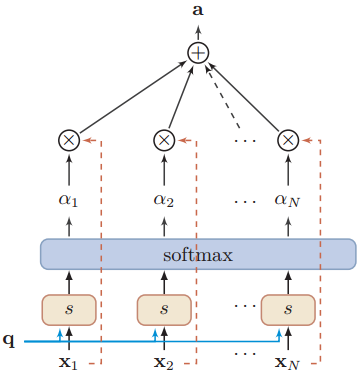
\includegraphics[width = 0.4\textwidth]{chapter2/attension.png}
    \caption{计算Attension值的过程图}
    \end{figure}

更一般的,可以用键值对(key-value pair)来表示输入信息,那么$N$个输入信息就可以表示为

\begin{equation}
	\begin{aligned}	
    (K, V)= [(k_1,v_1),(k_2,v_2),\ddots,(k_N,v_N)](K, V) \\
    &= [(k_1,v_1),(k_2,v_2),\ddots,(k_N,v_N)]
	\end{aligned}
\end{equation}

其中“键”用来计算注意分布$\alpha _i$,“值”用来计算聚合信息。
那么就可以将注意力机制看做是一种软寻址操作:把输入信息X看做是存储器中存储的内容,元素由地址Key(键)和值Value组成,当前有个Key=Query的查询,目标是取出存储器中对应的Value值,即Attention值。而在软寻址中,并非需要硬性满足Key=Query的条件来取出存储信息,而是通过计算Query与存储器内元素的地址Key的相似度来决定,从对应的元素Value中取出多少内容。每个地址Key对应的Value值都会被抽取内容出来,然后求和,这就相当于由Query与Key的相似性来计算每个Value值的权重,然后对Value值进行加权求和。加权求和得到最终的Value值,也就是Attention值。

以上的计算可以归纳为三个过程:根据Query和Key计算二者的相似度。可以用上面所列出的加性模型、点积模型或余弦相似度来计算,得到注意力得分$s_i$;
\begin{equation}
    s_i=F\left(Q, k_i\right)
    \end{equation}
用softmax函数对注意力得分进行数值转换。一方面可以进行归一化,得到所有权重系数之和为1的概率分布,另一方面可以用softmax函数的特性突出重要元素的权重;
\begin{equation}
    \alpha_i=\operatorname{softmax}\left(s_i\right)=\frac{\exp \left(s_i\right)}{\sum_{j=1}^N \exp \left(s_j\right)}
    \end{equation}
根据权重系数对Value进行加权求和:
\begin{equation}
    \operatorname{Attention}((K, V), Q)=\sum_{i=1}^N \alpha_i v_i
    \end{equation}

\begin{figure}[ht]
    \centering
    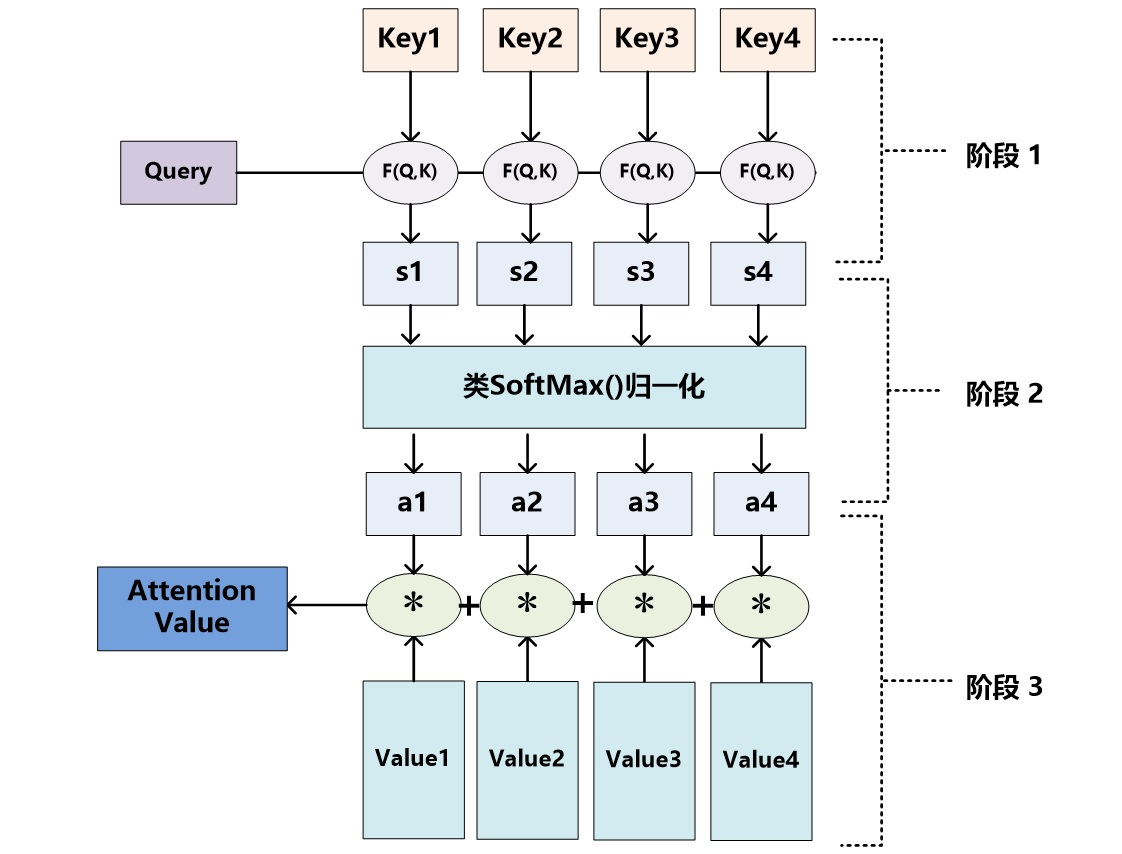
\includegraphics[width = 0.8\textwidth]{chapter2/attesion2.png}
    \caption{键值对注意力模式}
    \end{figure}
故可以得到整体注意力计算公式:
\begin{equation}
    \begin{aligned}
    \operatorname{att}((K, V), \mathbf{q}) &=\sum_{i=1}^N \alpha_i \mathbf{v}_i \\
    &=\sum_{i=1}^N \frac{\exp \left(s\left(\mathbf{k}_i, \mathbf{q}\right)\right)}{\sum_j \exp \left(s\left(\mathbf{k}_j, \mathbf{q}\right)\right)} \mathbf{v}_i
    \end{aligned}
    \end{equation}

%csdn https://blog.csdn.net/qq_37492509/article/details/114991482


\section{标准化流相关技术}
多年来,研究人员发明了许多方法来学习大型数据集的概率分布,包括生成对抗网络(GAN)\cite{gan}、变分自编码器(VAE)\cite{vae}和标准化流\cite{nf}等。GAN和VAE的能力本已十分惊人,它们都能通过简单的推理方法学习十分复杂的数据分布。然而,GAN和VAE都缺乏对概率分布的精确评估和推理,这往往导致VAE中的模糊结果质量不高,GAN训练也面临着如模式崩溃和后置崩溃等挑战。因此,Normalizing Flow应运而生,试图通过使用可逆函数来解决目前GAN和VAE存在的许多问题。

%原理
标准化流的核心思想是利用分布变换的可逆性 如果 $y=f(x)$, 且 $f$ 是可逆的, 则
\begin{equation}
    \begin{aligned}
        &p_x(x)=p_y(f(x)) *|\operatorname{det} J f(x)| \\
        &p_y(y)=p_x\left(f^{-1}(y)\right) *\left|\operatorname{det} J f^{-1}(y)\right|
        \end{aligned}
\end{equation}

当存在多个 $f$ 复合时, 可以在取log之后求和:
\begin{equation}
    \begin{aligned}
    \mathbf{z}_K &=f_K \circ \ldots \circ f_2 \circ f_1\left(\mathbf{z}_0\right) \\
    \log q_K\left(\mathbf{z}_K\right) &=\log q_0\left(\mathbf{z}_0\right)-\sum_{k=1}^K \log \operatorname{det}\left|\frac{\partial f_k}{\partial \mathbf{z}_k}\right|
    \end{aligned}
    \end{equation}

当前基于标准化流主要有三种实现方式,即,可加性耦合层\cite{nice},仿射耦合层\cite{realnvp},可逆的1x1卷积\cite{glow},其中可加性耦合层的做法:首先对于D维数据的 $x$, 将其随意地划分为两部分, $x_1, x_2$ ,并做变换:
\begin{equation}
    \begin{aligned}
        &\mathbf{y}_1=\boldsymbol{x}_1 \\
        &\mathbf{y}_2=\boldsymbol{x}_2+\boldsymbol{m}\left(\boldsymbol{x}_1\right)
        \end{aligned}
\end{equation}
其中m是一个任意的MLP函数, 通过这样的变换, 如果这个函数是可逆的, 即:
\begin{equation}
    \begin{aligned}
        &x_1=\mathbf{y}_1 \\
        &x_2=\mathbf{y}_2-\boldsymbol{m}\left(\boldsymbol{x}_1\right)
        \end{aligned}
\end{equation}

仿射耦合层提出了一种相对可加性耦合层复杂一点的方法, 即
\begin{equation}
    \begin{aligned}
        &\mathbf{y}_1=\boldsymbol{x}_1 \\
        &\mathbf{y}_2=\mathbf{s}\left(\mathbf{x}_1\right) \odot \boldsymbol{x}_2+t\left(\boldsymbol{x}_1\right)
        \end{aligned}
\end{equation}

通过乘一个非线性函数 $\mathbf{s}\left(\mathbf{x}_1\right)$, 本质上是一个线性变换。此处仿射耦合层的雅可比矩阵为:
\begin{equation}
    \frac{\partial \mathbf{y}}{\partial \mathbf{x}}=\left[\begin{array}{ll}
        \frac{\partial y_1}{\partial x_1} & \frac{\partial y_1}{\partial x_2} \\
        \frac{\partial y_2}{\partial x_1} & \frac{\partial y_2}{\partial x_2}
        \end{array}\right]=\left[\begin{array}{cc}
        \mathbb{I}_d & 0 \\
        \frac{\partial \mathbf{s}}{\partial \mathbf{x}_1} \otimes \mathbf{x}_2+\frac{\partial t}{\partial \mathbf{x}_1} & \operatorname{diag}(s)
        \end{array}\right]
\end{equation}

因为
\begin{equation}
    \left(\begin{array}{c}
        x_1 \\
        \vdots \\
        x_n
        \end{array}\right) \odot\left(\begin{array}{c}
        y_1 \\
        \vdots \\
        y_n
        \end{array}\right)=\left(\begin{array}{ccc}
        x_1 & \cdots & 0 \\
        \vdots & \ddots & \vdots \\
        0 & \cdots & x_n
        \end{array}\right)\left(\begin{array}{c}
        y_1 \\
        \vdots \\
        y_n
        \end{array}\right)
\end{equation}
所以在这里雅可比矩阵也是一个对角矩阵, 即$\frac{\partial y_2}{\partial x_2}=\frac{\partial \operatorname{diag}(\mathbf{s}) x_2}{\partial x_2}=\operatorname{diag}(\mathbf{s})$。

可逆的1x1卷积做法是将一个卷积核表达成一个矩阵乘积, 即可以写出一个矩阵的计算公式:$Y=XW$
比如, $x$ 是 $h * w * c$ 的张量, $\mathrm{c}$ 表示channel, 对于1x1卷积来说, W就是一个 $c * c$ 的矩阵, 就是他们的乘积, 实际上可以将x当成 $h * w$ 行 $c$ 列的矩阵, 乘以W。
利用LU分解,构造一个一定可逆的矩阵 $W$。因为任意矩阵都可以表达成$W=PLU$

其中P是置换矩阵, $\mathrm{L}$ 是下三角矩阵, 对角线元素全为 $1, \mathrm{U}$ 是上三角矩阵, 为了保证矩阵 $W$ 可逆, 需要保证 $P , L$, U满秩, 又因为 $P$, L一定是满秩的, 所以只要保证 $U$ 满秩即可。那么 一个方便的方法就是:
\begin{equation}
    W=P L(U+\operatorname{diag}(s))
\end{equation}
其中, U是严格上三角矩阵, 其对角线为 0, 最终可逆卷积核其导数行列式的求解为:
\begin{equation}
    \begin{aligned}
        &\log \left|\operatorname{det}\left(\frac{d \operatorname{conv} 2 \mathrm{D}(\mathbf{h} ; \mathbf{W})}{d \mathbf{h}}\right)\right|=h \cdot w \cdot \log |\operatorname{det}(\mathbf{W})| \\
        &=h \cdot w \cdot \log |\operatorname{diag}(s)|=h \cdot w \cdot \operatorname{sum}(\log (|s|))
        \end{aligned}
\end{equation}

\section{本章小结}
本章是缺失值时间序列异常检测技术的相关理论基础。首先介绍了什么是时间序列中的异常,即时间序列异常的相关类型,包括点异常,上下文异常,集合异常和其他异常等。然后有关时间序列相关特性,即时间序列的相关属性,包括时序性,维度,非平稳性,噪声等属性。之后介绍了有关注意力机制相关技术,首先介绍了注意力机制的基本原理,然后介绍了注意力机制的计算方式及公式。最后介绍了标准化流的相关技术,包括当前主流实现标准化流的几种方式,即可加性耦合层,仿射耦合层等。